\documentclass[12pt]{article}

\usepackage{graphicx}
\usepackage{epstopdf}
\usepackage[english]{babel}
\usepackage[latin5]{inputenc}
\usepackage{hyperref}
\usepackage[left=3cm,top=3cm,right=3cm,bottom=2cm,nohead,nofoot]{geometry}
\usepackage{datenumber}

\begin{document}

\begin{center}
\Huge
Project: Enigma Machine and Turing-Welchman Bombe

\vspace{10mm}
\Large
Maria Camila REMOLINA GUTI�RREZ
\large
maria.remolina\_gutierrez@telecom-sudparis.eu

\vspace{5mm}
\Large
Advisor: Prof. Eric RENAULT

\vspace{5mm}
\normalsize
\today
\end{center}

\vspace{5mm}
\begin{abstract}
	This is the work proposal to follow in the course Project as part of the master M1 in Computer Science and Communication Networks at T�l�com SudParis. The goal is to implement the Enigma machine used in World War II, followed by the Bombe machine that breaks the cipher, created by Alan Turing and Gordon Welchman at Bletchley Park.
\end{abstract}


\section{Introduction}

The enigma machine is a cipher machine used by the Nazi Germany during World War II in order to send secret coded messages. It was initially a commercial machine bought by banks are businesses. But then the military took it and added an extra security layer called plugboard. It was innovative at the time because it was not a substitution cipher, i.e. the same letter can get different results after encryption. \\

The machine works by a combination of moving rotors and inside wiring as seen in Fig. \ref{fig:machine}. The way to use it is that when the sender types a message, a bulb lights up indicating the correspondent coded letter. Then, in order to decode, the receiver types the coded message he received and the initial message lights up on the board. In war times the coded messages were transmitted over morse code. \\

\begin{figure}[h!]
	\centering
	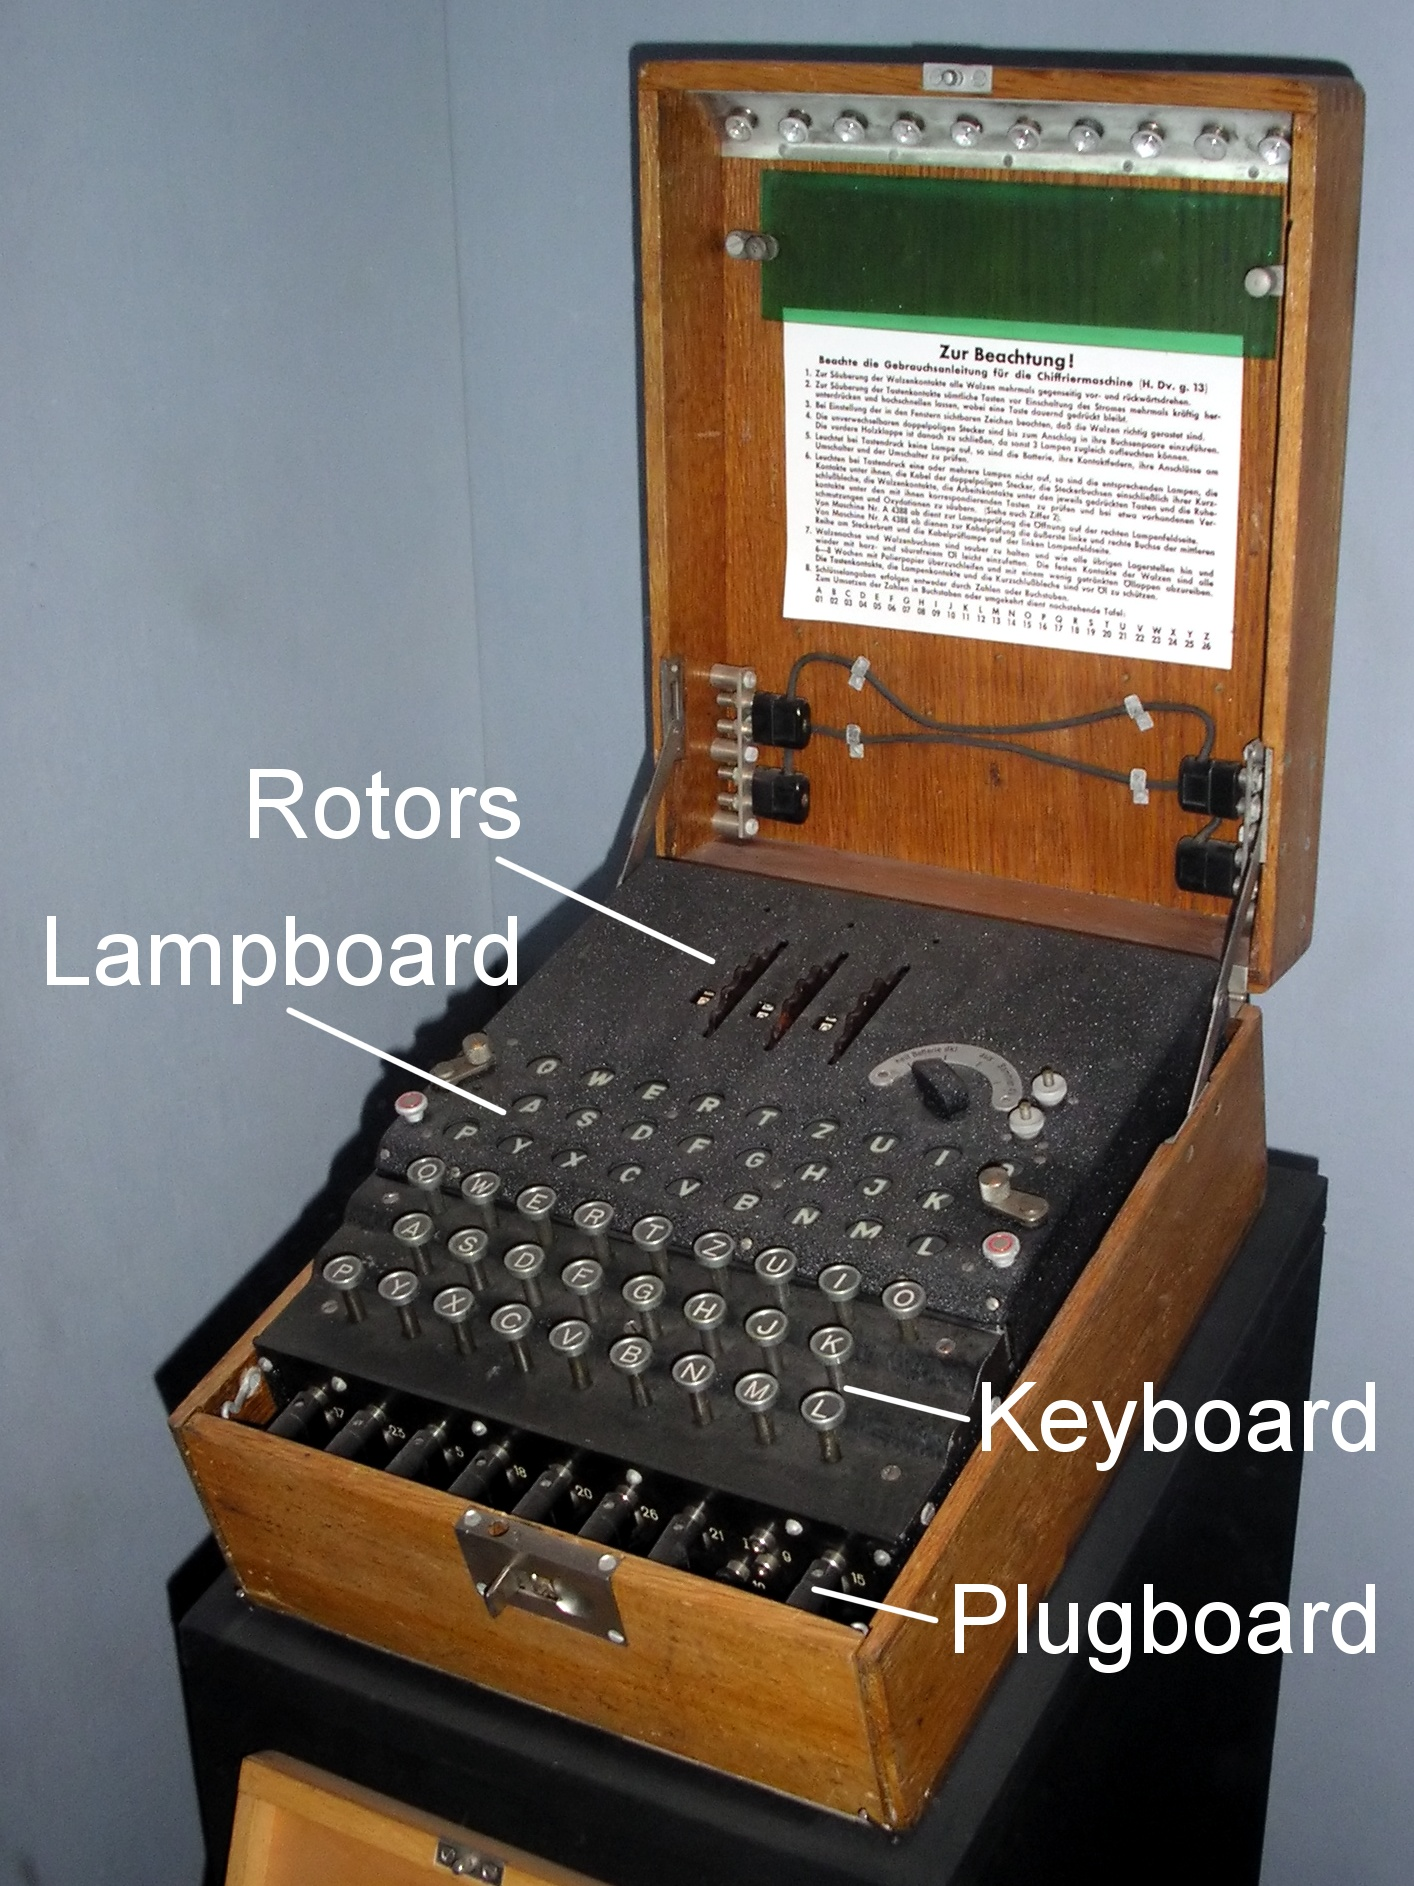
\includegraphics[width=0.5\textwidth]{img/machine}
	\caption{Enigma Machine - Military Edition}
	\label{fig:machine}
\end{figure}

In the military version of the Enigma Machine there were 5 possible rotors to pick from, each with 26 possible positions, then there were 10 possible switching in the plugboard that could choose a pair from the available 26 letters. That accounts for $158962555217826360000$ different combinations for
the setting of the army Enigma Machine \cite{numberphile1}. The initial setting for each day was given to the bases in a sheet of paper that had the monthly configurations of the machine. So they changed the setting everyday. \\

So in order to decipher the code, you needed either to have the code sheet or to break the message. This latter was what the scientists at Bletchley Park did; and what I will try to recreate in this project. 

\section{General Goal}

To understand the code breaking process behind the enigma cipher.


\section{Specific Goals}

\begin{itemize}
	\item To implement the Enigma machine with software
	\item To implement the Bombe machine that breaks the Enigma cipher
	\item To understand the mathematical and probabilistic techniques used to break a cipher with limited time and computational resources. 
	\item To understand the weaknesses exploited that allowed to break the Enigma cipher
\end{itemize}


\section{Methodology}

I created 2 different programs within the same project: 

\begin{enumerate}
	\item The Enigma machine 
	\item The Bombe machine
\end{enumerate}

The implementation of both is in Python and it is be publicly available in the GitHub repository \url{https://github.com/mariacamilarg/enigma_bombe}. As for the computational resources, I used only my personal computer (running a Linux O.S.) with standard architecture.


\section{Results}

\subsection{Enigma Machine}

There are different models of the Enigma machine that were developed through time. In this project I chose one of the latest, i.e. with more complicated settings. This is the model M3 \& M4 Naval (from Frebuary 1942) that has 8 possible rotors \cite{dade,wikirotors}. 

\subsubsection{Input}

\subsubsection{Processing}

\subsubsection{Output}

\subsubsection{Challenges}

The biggest challenge in implementing the Enigma machine is knowing exactly how it worked. Even thought there is a great amount of information online, the depth of it is not that significant. Most of the resources tend to shallowly explain the behavior but there are several subtleties and details that were hard to find. I put in the references the most trustworthy and complete information I found on the matter \cite{rijmenants,sale,cryptomuseum,wiki,wikicryptanalysis,ellsbury}. \\

Another challenge was the translation of this information, because the original machine settings are in German. This implies that there are multiple acceptable translations for several parts of the machine that might be opposite among different sources. A concrete example of this goes within the rotor, where there are 2 different settings called \textit{Ringstellung} and \textit{Grundstellung}. They refer to the ring setting within each the rotor and to the ground setting or offset of the rotor within the machine, respectively. However figuring out which one was which presented a problem because different sources referred to them by different names, sometimes even opposite. So I had to solve this by recurring to the German words. \\

Finally, I would like to refer as well to different simulators that are found on the internet in which I could get a phenomenological understanding of the machine. I was able to try out different configurations and learning its way to function. I also confirmed my solution against these simulators in order to test my implementation. This was a positive match. 

\begin{itemize}
	\item Cryptii Simulator: \url{https://cryptii.com/pipes/enigma-machine}
	\item Louise Dade Simulator: \url{http://enigma.louisedade.co.uk/enigma.html}
\end{itemize}


\subsection{Bombe Machine}




\begin{thebibliography}{10}
% -- enigma --
	\bibitem{hodges} A. Hodges. \textit{Alan Turing: The Enigma}. Princeton, N.J: Princeton University Press (2012). 
	\bibitem{numberphile1} Numberphile. \textit{158,962,555,217,826,360,000 (Enigma Machine)}. YouTube (2013). % https://www.youtube.com/watch?v=G2_Q9FoD-oQ
	\bibitem{rijmenants} D. Rijmenants. \textit{Technical Details of the Enigma Machine}. Obtained from: \url{http://users.telenet.be/d.rijmenants/en/enigmatech.htm}
	\bibitem{sale} T. Sale. \textit{Military Use of the Enigma}. Obtained from: \url{https://www.codesandciphers.org.uk/enigma/enigma3.htm}
	\bibitem{cryptomuseum} Cryptomuseum. \textit{Enigma Cipher Machines}. Obtained from: \url{https://www.cryptomuseum.com/crypto/enigma/index.htm}	
	\bibitem{wiki} Wikipedia. \textit{Enigma Machine}. Obtained from: \url{https://en.wikipedia.org/wiki/Enigma_machine}
	\bibitem{wikicryptanalysis} Wikipedia. \textit{Cryptanalysis of the Enigma}. Obtained from: \url{https://en.wikipedia.org/wiki/Cryptanalysis_of_the_Enigma}
	
	\bibitem{dade} L. Dade. \textit{Enigma Machine: How It Works}. Obtained from: \url{http://enigma.louisedade.co.uk/howitworks.html}
	\bibitem{wikirotors} Wikipedia. \textit{Enigma Rotor Details}. Obtained from: \url{https://en.wikipedia.org/wiki/Enigma_rotor_details}
	
% -- bombe --
	\bibitem{ellsbury} G. Ellsbury. \textit{The Enigma and The Bombe}. Obtained from: \url{http://www.ellsbury.com/enigmabombe.htm}
\end{thebibliography}


\end{document} 